\chapter{Практическая часть}

Ниже представленны листинги программы:

\lstset{language=python}
\begin{lstlisting}[caption=Интерполяция]
def interpolation(val, tableVal, table):
    min_i = 0
    max_i = 0

    for i in range(len(tableVal)):
        if (val > tableVal[i]):
            max_i = i
        else:
            max_i = i
            break

    if (0 == max_i):
        max_i = 1

    min_i = max_i - 1

    return table[min_i] + (table[max_i] - table[min_i]) / (tableVal[max_i] - tableVal[min_i]) * (val - tableVal[min_i])

\end{lstlisting}

\lstset{language=python}
\begin{lstlisting}[caption=Интегрирование методом трапеций]
def funcInt(I, z):
    t0 = interpolation(I, table_I, table_T0)
    global gt0
    gt0 = t0
    m = interpolation(I, table_I, table_M)
    t = t0 + (tw - t0) * (z ** m)

    sigma = interpolation(t, table_T, table_Sigma)

    return sigma * z

def trapezoidInt(I):
    a = 0
    b = 1
    n = 100
    h = (b - a) / n

    s = (funcInt(I, a) + funcInt(I, b)) / 2

    x = 0
    for i in range(n - 1):
        x = x + h
        s = s + funcInt(I, x)

    s = s * h
    return s
\end{lstlisting}

\lstset{language=python}
\begin{lstlisting}[caption=Нахождение сопротивления]
def Rp(le, R, I):
    return le / (2 * pi * R ** 2 * trapezoidInt(I))
\end{lstlisting}

\lstset{language=python}
\begin{lstlisting}[caption=Решение системы уравнений методом Рунге-Кутта 2-го и 4-го порядка]
def f(I, U, le, R, Lk, Rk):
    global grp
    grp = Rp(le, R, fabs(I))

    return (U - (Rk + grp) * I) / Lk

def g(I, Ck):
    return -I / Ck

def stepOrder4(I, U, le, R, Lk, hn, Rk, Ck):
    k1 = f(I, U, le, R, Lk, Rk)
    q1 = g(I, Ck)

    k2 = f(I + hn * k1 / 2, U + hn * q1 / 2, le, R, Lk, Rk)
    q2 = g(I + hn * k1 / 2, Ck)

    k3 = f(I + hn * k2 / 2, U + hn * q2 / 2, le, R, Lk, Rk)
    q3 = g(I + hn * k2 / 2, Ck)

    k4 = f(I + hn * k3, U + hn * q3, le, R, Lk, Rk)
    q4 = g(I + hn * k3, Ck)

    return I + hn * (k1 + 2 * k2 + 2 * k3 + k4) / 6, U + hn * (q1 + 2 * q2 + 2 * q3 + q4) / 6

def stepOrder2(I, U, le, R, Lk, hn, Rk, Ck):
    k1 = f(I, U, le, R, Lk, Rk)
    q1 = g(I, Ck)

    k2 = f(I + hn * k1 / 2, U + hn * q1 / 2, le, R, Lk, Rk)
    q2 = g(I + hn * k1 / 2, Ck)

    return I + hn * ((1 - alpha) * k1 + alpha * k2), U + hn * ((1 - alpha) * q1 + alpha * q2)
\end{lstlisting}

\newpage

На изображениях ниже представлены скриншот работы программы:
\begin{figure}[H]
    \centering
    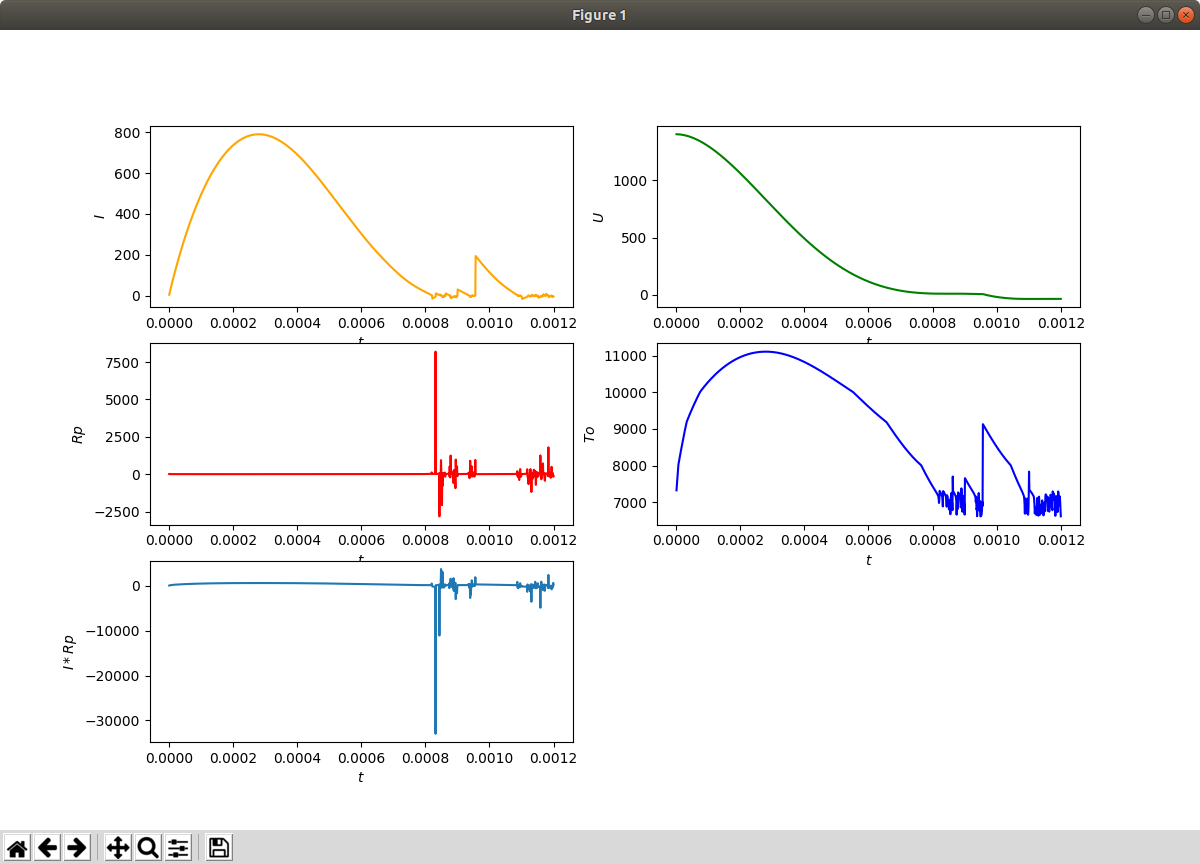
\includegraphics[scale=0.4]{data/image/work.png}
    \caption{Результат работы метода Рунге-Кутта 2-го порядка.}
\end{figure}

\begin{figure}[H]
    \centering
    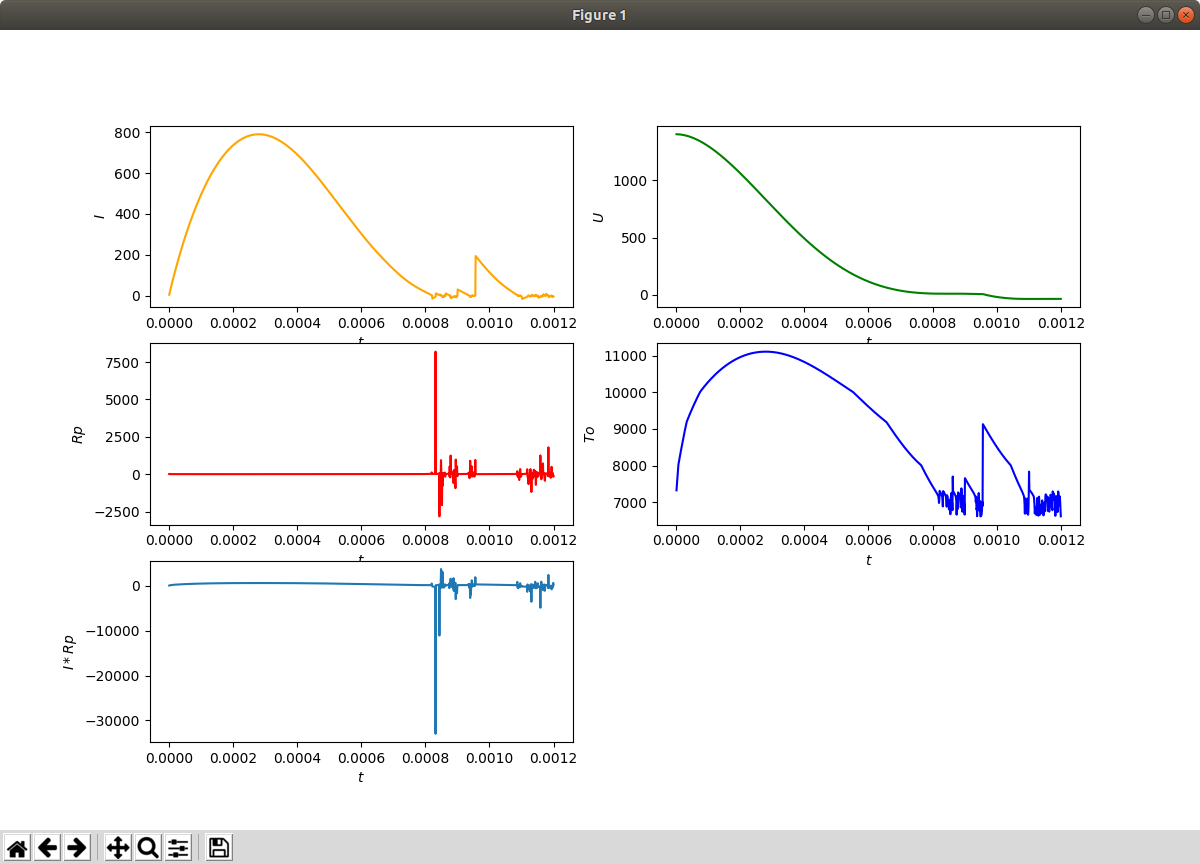
\includegraphics[scale=0.4]{data/image/work.png}
    \caption{Результат работы метода Рунге-Кутта 4-го порядка.}
\end{figure}
